\section{Additional figures}

\subsection{Additional summer days}
\begin{figure}[h!]
    \centering
    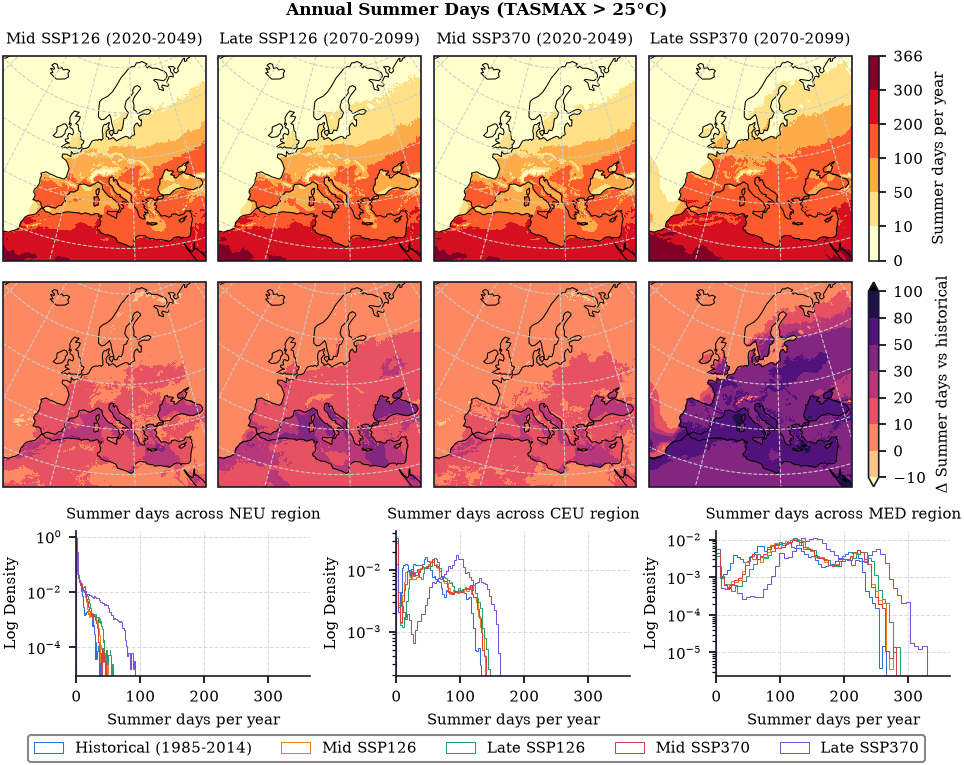
\includegraphics[width=0.5\linewidth]{figures/data_section/climatology/summer_days_hclim_r1i1p1f1.png}
    \caption{Annual summer days in the \gls{hclim} data for \gls{realisation} one. Annual summer days is defined as the number of days in which tasmax exceeds 25°C. The top row shows the absolute number of annual summer days for \gls{126} (mid and late century) and \gls{370} (mid and late century). The middle row shows the change in annual summer days to the historical reference period (i.e. the change in climate). The last row shows the distribution of annual summer days in the three IPCC regions (see \href{https://interactive-atlas.ipcc.ch/regional-information}{here}).}
    \label{fig:summer_days_r1}
\end{figure}

\begin{figure}[h!]
    \centering
    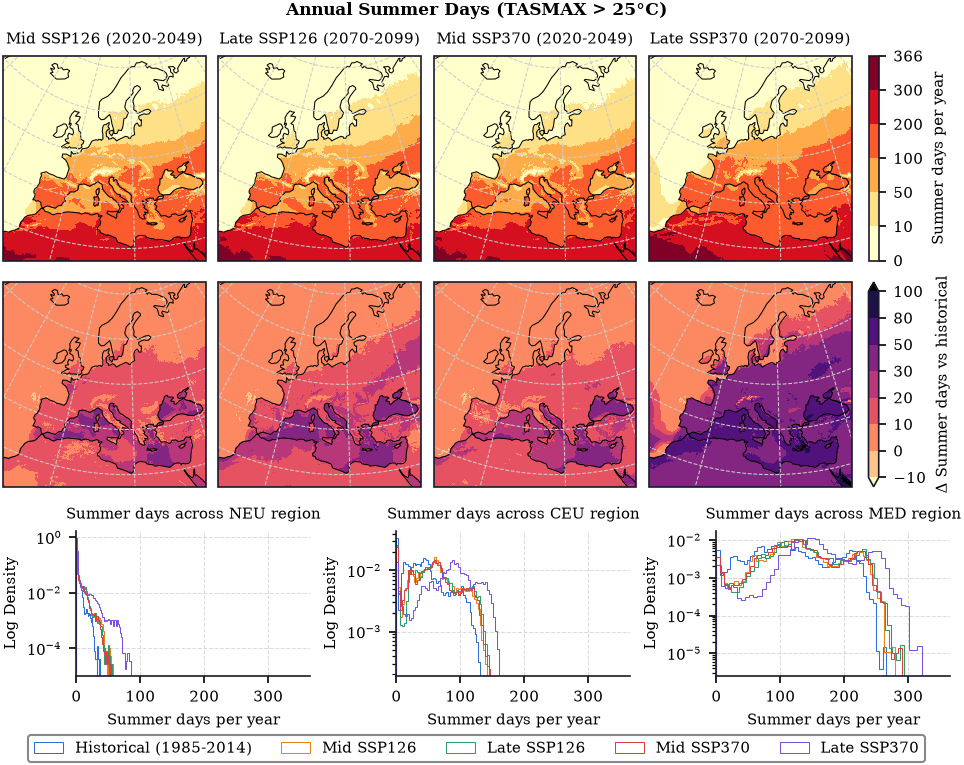
\includegraphics[width=0.5\linewidth]{figures/data_section/climatology/summer_days_hclim_r2i1p1f1.png}
    \caption{Annual summer days in the \gls{hclim} data for \gls{realisation} two. Annual summer days is defined as the number of days in which tasmax exceeds 25°C. The top row shows the absolute number of annual summer days for \gls{126} (mid and late century) and \gls{370} (mid and late century). The middle row shows the change in annual summer days to the historical reference period (i.e. the change in climate). The last row shows the distribution of annual summer days in the three IPCC regions (see \href{https://interactive-atlas.ipcc.ch/regional-information}{here}).}
    \label{fig:summer_days_r2}
\end{figure}

\subsection{Additional frost days}
\begin{figure}[tb]
    \centering
    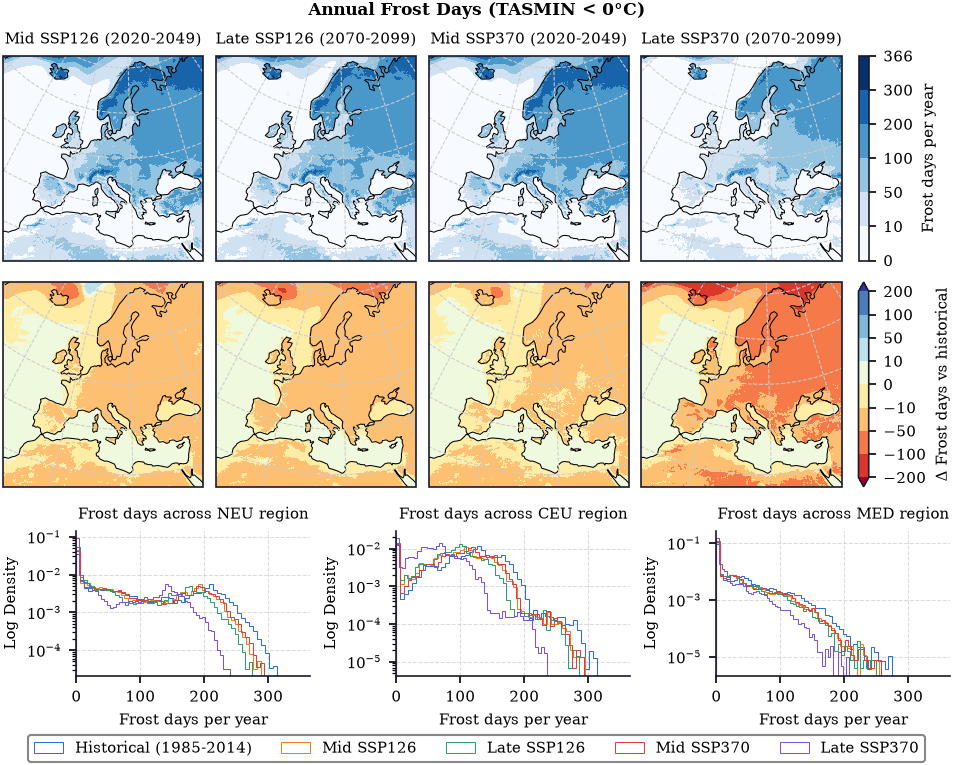
\includegraphics[width=0.5\linewidth]{figures/data_section/climatology/frost_days_hclim_r1i1p1f1.png}
    \caption{Annual frost days in the \gls{hclim} domain for \gls{realisation} one. Annual frost days are defined as the number of days in which the daily minimum temperature (tasmin) subceeds 0°C. The top row shows the mean number of annual frost days for \gls{126} (mid and late century) and \gls{370} (mid and late century). The middle row shows the change in annual frost days to the historical reference period (i.e. the change in climate). The last row shows the distribution of annual frost days in the three IPCC regions (see \href{https://interactive-atlas.ipcc.ch/regional-information}{here}).}
    \label{fig:frost_days_r1}
\end{figure}

\begin{figure}[tb]
    \centering
    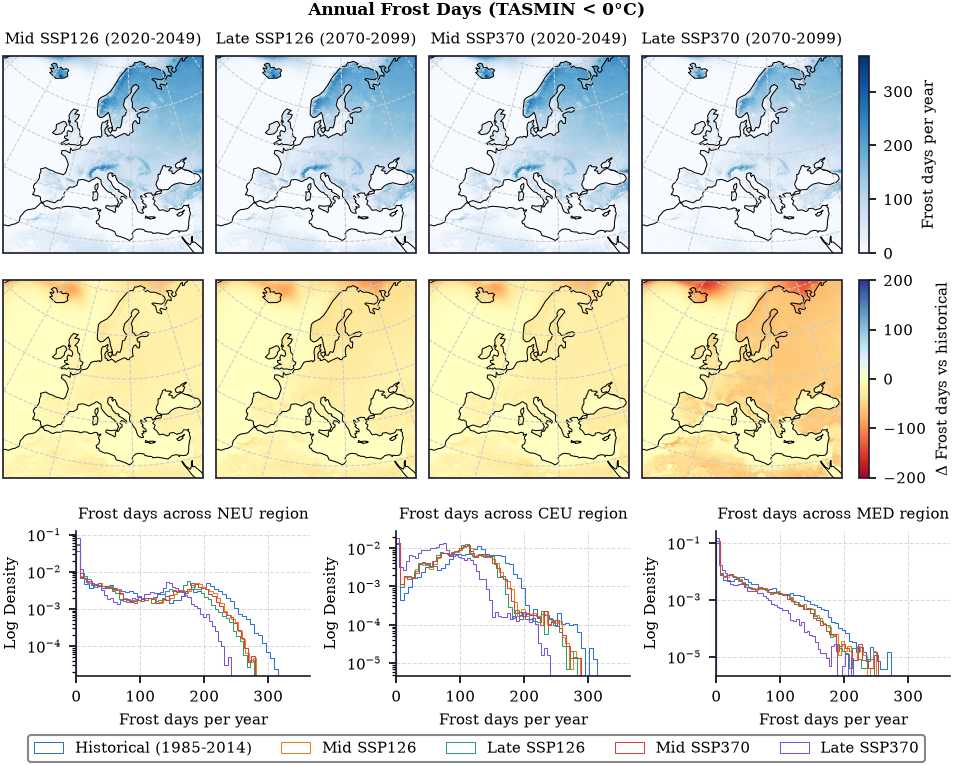
\includegraphics[width=0.5\linewidth]{figures/data_section/climatology/frost_days_hclim_r2i1p1f1.png}
    \caption{Annual frost days in the \gls{hclim} domain for \gls{realisation} two. Annual frost days are defined as the number of days in which the daily minimum temperature (tasmin) subceeds 0°C. The top row shows the mean number of annual frost days for \gls{126} (mid and late century) and \gls{370} (mid and late century). The middle row shows the change in annual frost days to the historical reference period (i.e. the change in climate). The last row shows the distribution of annual frost days in the three IPCC regions (see \href{https://interactive-atlas.ipcc.ch/regional-information}{here}).}
    \label{fig:frost_days_r2}
\end{figure}

\subsection{Additional wet days}

\begin{figure}[tb]
    \centering
    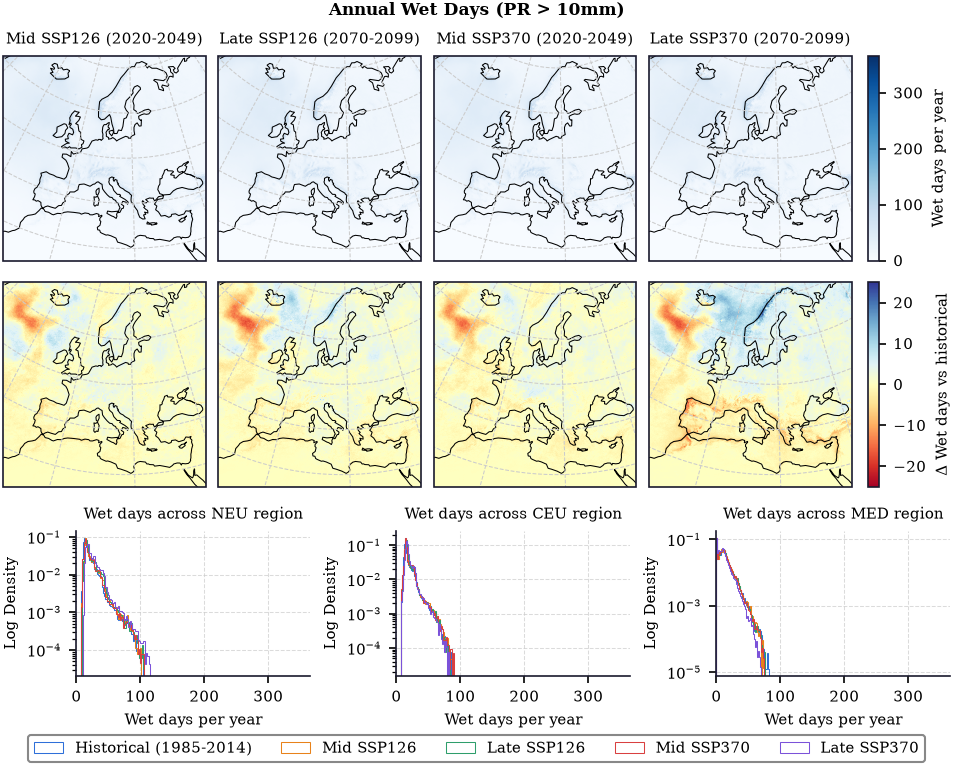
\includegraphics[width=0.5\linewidth]{figures/data_section/climatology/wet_days_hclim_r1i1p1f1.png}
    \caption{Annual wet days in the \gls{hclim} domain for \gls{realisation} one. Annual wet days are defined as the number of days in which the total precipitation exceeds $10 \frac{kg}{m^2} \approx 10 mm$. The top row shows the mean number of annual wet days for \gls{126} (mid and late century) and \gls{370} (mid and late century). The middle row shows the change in annual wet days to the historical reference period (i.e. the change in climate). The last row shows the distribution of annual wet days in the three IPCC regions (see \href{https://interactive-atlas.ipcc.ch/regional-information}{here}).}
    \label{fig:wet_days_r1}
\end{figure}

\begin{figure}[tb]
    \centering
    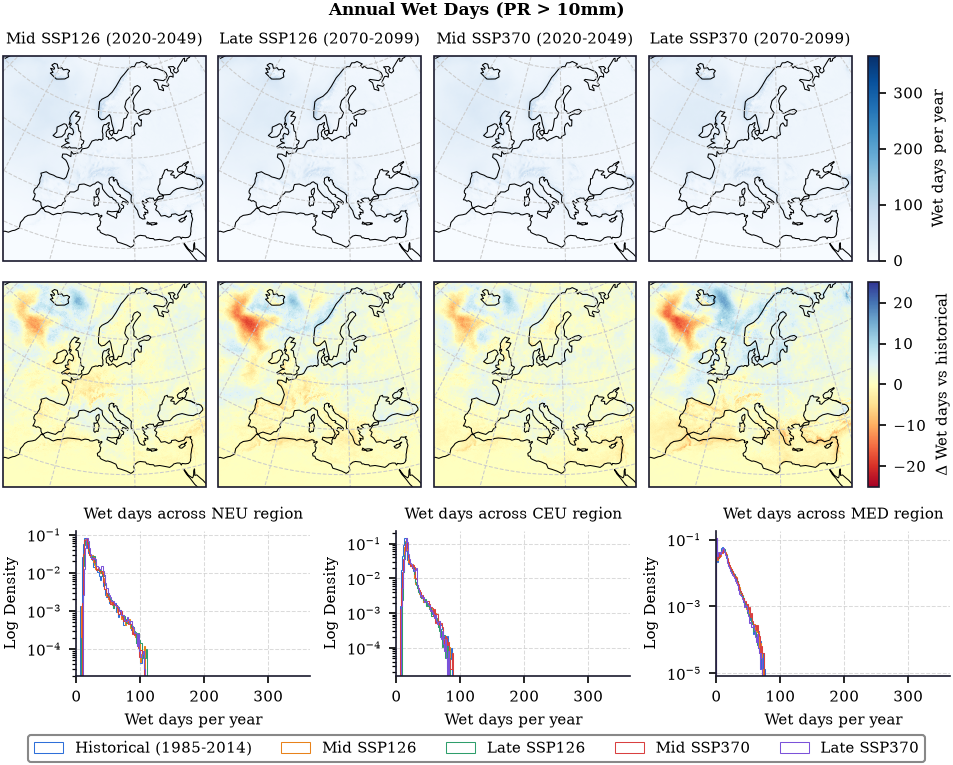
\includegraphics[width=0.5\linewidth]{figures/data_section/climatology/wet_days_hclim_r2i1p1f1.png}
    \caption{Annual wet days in the \gls{hclim} domain for \gls{realisation} two. Annual wet days are defined as the number of days in which the total precipitation exceeds $10 \frac{kg}{m^2} \approx 10 mm$. The top row shows the mean number of annual wet days for \gls{126} (mid and late century) and \gls{370} (mid and late century). The middle row shows the change in annual wet days to the historical reference period (i.e. the change in climate). The last row shows the distribution of annual wet days in the three IPCC regions (see \href{https://interactive-atlas.ipcc.ch/regional-information}{here}).}
    \label{fig:wet_days_r2}
\end{figure}